\subsection{Fazit}

\begin{frame}{Fazit}

	\pause
	Wir hatten
	\pause
	\begin{itemize}
		\item Ziemlich viel Arbeit
		\pause
		\item Einige Coding-Marathons
		\pause
		\item Mindestens 5 Nervenzusammenbr\"uche wegen des c++ 11 Standards
		\pause
		\item Mindestens 20 Nervenzusammenbr\"uche weil jemand auf die Idee gekommen ist Eclipse zu verwenden
		\pause
		\item Noch ein paar Nervenzusammenbr\"uche mehr wegen der Fehlermeldungen des GCC
		\pause
		\item \"Uber 20 Mal "Oh Nein, das Projekt kompiliert nicht mehr!"
		\pause
		\item Mindestens 4 Wochen lang eine kaputte .class-Datei generiert
		\pause
		\item Zahllose Wtf-Momente
	\end{itemize}

\end{frame}

\begin{frame}{Fazit}

	\pause
	Außerdem haben/hatten wir:
	\pause
	\begin{itemize}
		\item Viel gelernt
		\pause
		\item Ziemlich viel Spaß gehabt
		\pause
		\item Super Teamgeist bewiesen
		\pause
		\item Regelm\"aßig Kekse gegessen
		\pause
		\item Also kurz: Spiel, Spaß und Schokolade
		\pause
	\end{itemize} \newline \newline \vspace{5mm}	\textbf{\textcolor{fu-green}{Also auch wenn wir das Projekt Jail++ getauft haben	kam uns das Projekt nicht wie ein Gef\"angnisaufenthalt vor.}}
	
	\begin{figure}
		  \begin{center}
		    \leavevmode
		      
\includegraphics[width = .2\textwidth]{smiley}
		  \end{center}
		\end{figure}
	
\end{frame}

\begin{frame}{Fazit}

	\begin{figure}
	  \begin{center}
	    \leavevmode
	      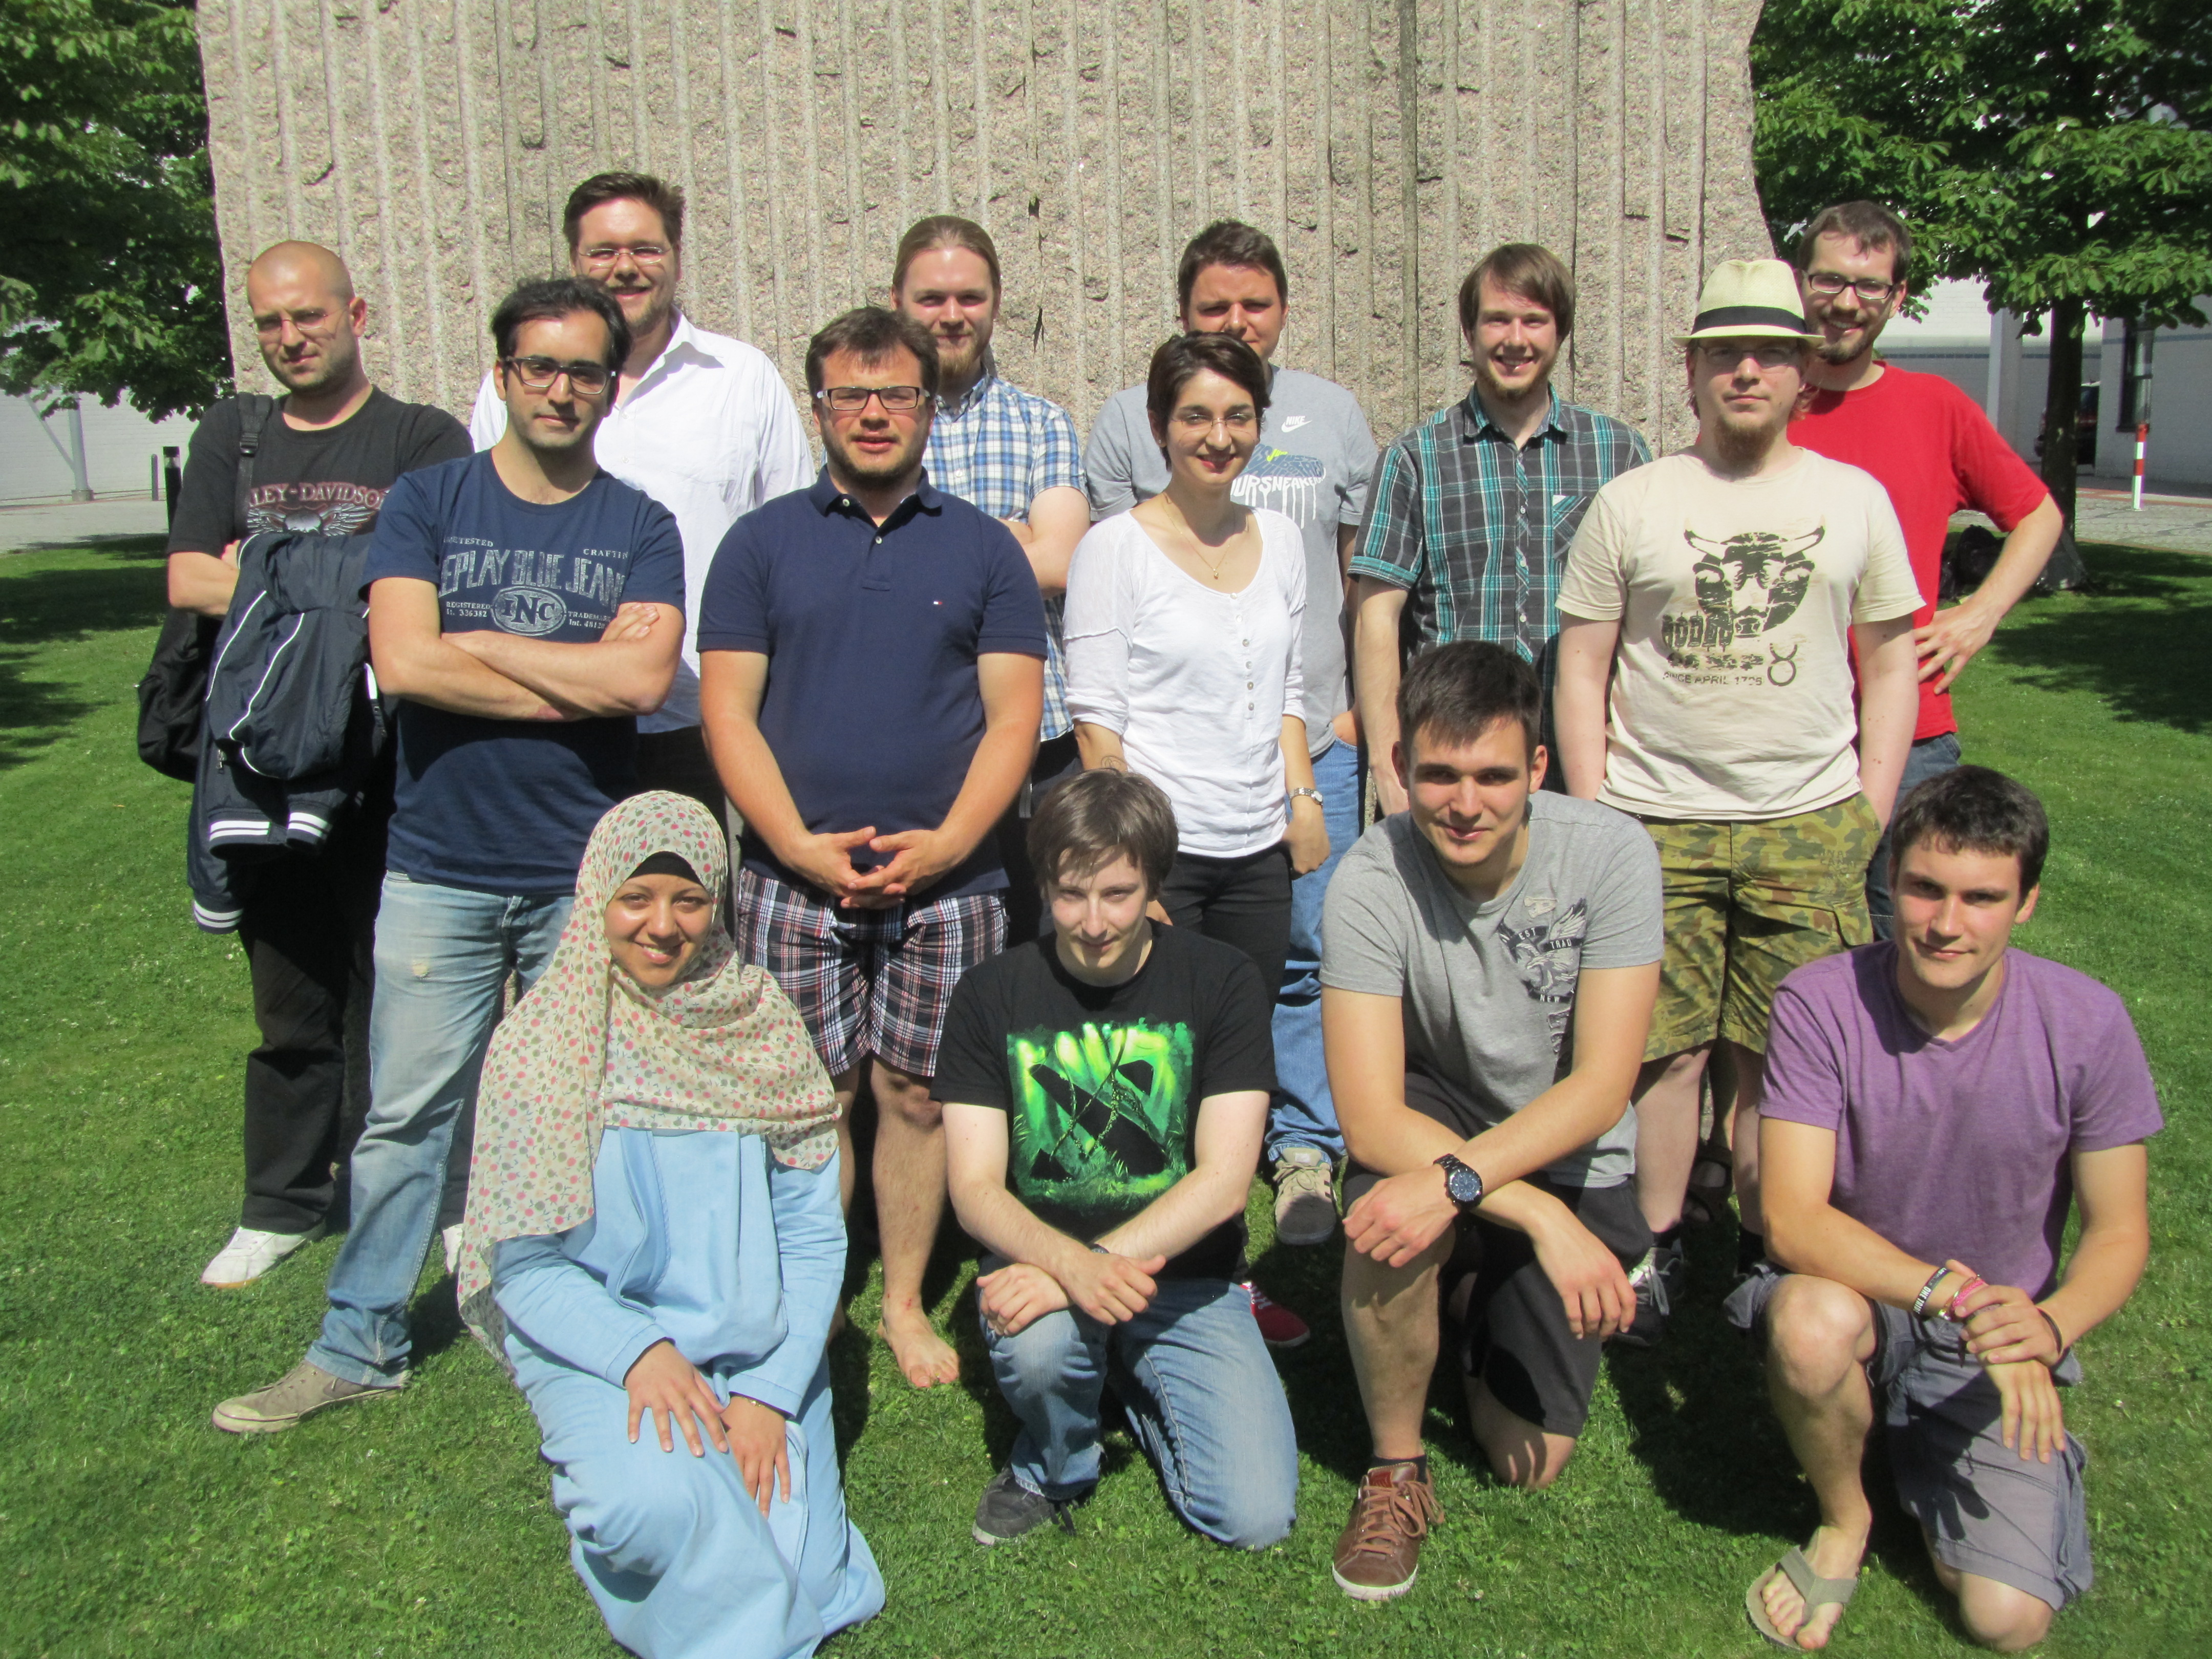
\includegraphics[width = .75\textwidth]{gruppe}
	    \caption{Jail Constructions Ltd. (auch bekannt als C++ Gruppe)}
	  \end{center}
	\end{figure}

\end{frame}